% Created by tikzDevice version 0.10.1 on 2016-08-15 14:38:24
% !TEX encoding = UTF-8 Unicode
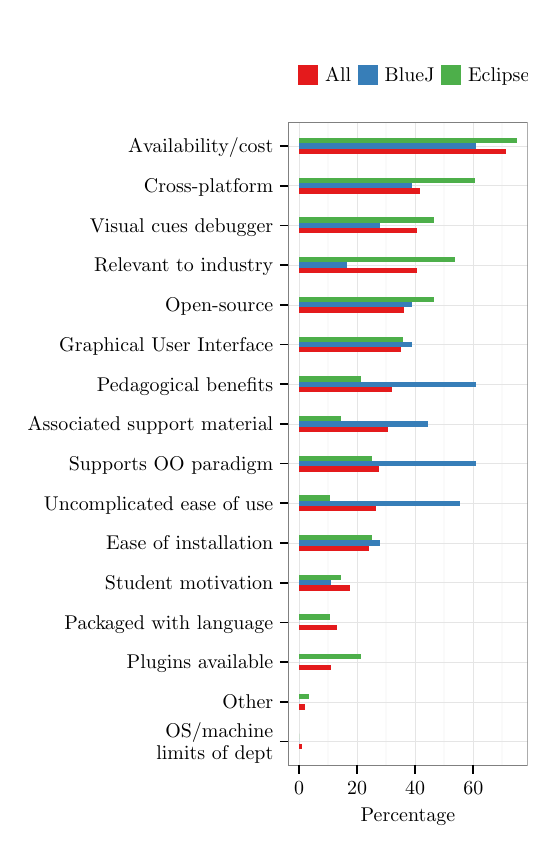
\begin{tikzpicture}[x=1pt,y=1pt]
\definecolor{fillColor}{RGB}{255,255,255}
\path[use as bounding box,fill=fillColor,fill opacity=0.00] (0,0) rectangle (180.67,289.08);
\begin{scope}
\path[clip] (  0.00,  0.00) rectangle (180.67,289.08);
\definecolor{drawColor}{RGB}{255,255,255}
\definecolor{fillColor}{RGB}{255,255,255}

\path[draw=drawColor,line width= 0.6pt,line join=round,line cap=round,fill=fillColor] (  0.00,  0.00) rectangle (180.68,289.08);
\end{scope}
\begin{scope}
\path[clip] ( 94.14, 22.52) rectangle (180.67,254.94);
\definecolor{fillColor}{RGB}{255,255,255}

\path[fill=fillColor] ( 94.14, 22.52) rectangle (180.67,254.94);
\definecolor{drawColor}{gray}{0.98}

\path[draw=drawColor,line width= 0.6pt,line join=round] (108.56, 22.52) --
	(108.56,254.94);

\path[draw=drawColor,line width= 0.6pt,line join=round] (129.54, 22.52) --
	(129.54,254.94);

\path[draw=drawColor,line width= 0.6pt,line join=round] (150.52, 22.52) --
	(150.52,254.94);

\path[draw=drawColor,line width= 0.6pt,line join=round] (171.50, 22.52) --
	(171.50,254.94);
\definecolor{drawColor}{gray}{0.90}

\path[draw=drawColor,line width= 0.2pt,line join=round] ( 94.14, 31.13) --
	(180.67, 31.13);

\path[draw=drawColor,line width= 0.2pt,line join=round] ( 94.14, 45.47) --
	(180.67, 45.47);

\path[draw=drawColor,line width= 0.2pt,line join=round] ( 94.14, 59.82) --
	(180.67, 59.82);

\path[draw=drawColor,line width= 0.2pt,line join=round] ( 94.14, 74.17) --
	(180.67, 74.17);

\path[draw=drawColor,line width= 0.2pt,line join=round] ( 94.14, 88.51) --
	(180.67, 88.51);

\path[draw=drawColor,line width= 0.2pt,line join=round] ( 94.14,102.86) --
	(180.67,102.86);

\path[draw=drawColor,line width= 0.2pt,line join=round] ( 94.14,117.21) --
	(180.67,117.21);

\path[draw=drawColor,line width= 0.2pt,line join=round] ( 94.14,131.55) --
	(180.67,131.55);

\path[draw=drawColor,line width= 0.2pt,line join=round] ( 94.14,145.90) --
	(180.67,145.90);

\path[draw=drawColor,line width= 0.2pt,line join=round] ( 94.14,160.25) --
	(180.67,160.25);

\path[draw=drawColor,line width= 0.2pt,line join=round] ( 94.14,174.59) --
	(180.67,174.59);

\path[draw=drawColor,line width= 0.2pt,line join=round] ( 94.14,188.94) --
	(180.67,188.94);

\path[draw=drawColor,line width= 0.2pt,line join=round] ( 94.14,203.29) --
	(180.67,203.29);

\path[draw=drawColor,line width= 0.2pt,line join=round] ( 94.14,217.63) --
	(180.67,217.63);

\path[draw=drawColor,line width= 0.2pt,line join=round] ( 94.14,231.98) --
	(180.67,231.98);

\path[draw=drawColor,line width= 0.2pt,line join=round] ( 94.14,246.33) --
	(180.67,246.33);

\path[draw=drawColor,line width= 0.2pt,line join=round] ( 98.07, 22.52) --
	( 98.07,254.94);

\path[draw=drawColor,line width= 0.2pt,line join=round] (119.05, 22.52) --
	(119.05,254.94);

\path[draw=drawColor,line width= 0.2pt,line join=round] (140.03, 22.52) --
	(140.03,254.94);

\path[draw=drawColor,line width= 0.2pt,line join=round] (161.01, 22.52) --
	(161.01,254.94);
\definecolor{fillColor}{RGB}{228,26,28}

\path[fill=fillColor] ( 98.07, 28.26) rectangle ( 99.23, 30.17);
\definecolor{fillColor}{RGB}{77,175,74}

\path[fill=fillColor] ( 98.07, 32.08) rectangle ( 98.07, 34.00);
\definecolor{fillColor}{RGB}{55,126,184}

\path[fill=fillColor] ( 98.07, 30.17) rectangle ( 98.07, 32.08);
\definecolor{fillColor}{RGB}{228,26,28}

\path[fill=fillColor] ( 98.07, 42.60) rectangle (100.38, 44.52);
\definecolor{fillColor}{RGB}{77,175,74}

\path[fill=fillColor] ( 98.07, 46.43) rectangle (101.82, 48.34);
\definecolor{fillColor}{RGB}{55,126,184}

\path[fill=fillColor] ( 98.07, 44.52) rectangle ( 98.07, 46.43);
\definecolor{fillColor}{RGB}{228,26,28}

\path[fill=fillColor] ( 98.07, 56.95) rectangle (109.60, 58.86);
\definecolor{fillColor}{RGB}{77,175,74}

\path[fill=fillColor] ( 98.07, 60.78) rectangle (120.55, 62.69);
\definecolor{fillColor}{RGB}{55,126,184}

\path[fill=fillColor] ( 98.07, 58.86) rectangle ( 98.07, 60.78);
\definecolor{fillColor}{RGB}{228,26,28}

\path[fill=fillColor] ( 98.07, 71.30) rectangle (111.91, 73.21);
\definecolor{fillColor}{RGB}{77,175,74}

\path[fill=fillColor] ( 98.07, 75.12) rectangle (109.31, 77.04);
\definecolor{fillColor}{RGB}{55,126,184}

\path[fill=fillColor] ( 98.07, 73.21) rectangle ( 98.07, 75.12);
\definecolor{fillColor}{RGB}{228,26,28}

\path[fill=fillColor] ( 98.07, 85.64) rectangle (116.51, 87.56);
\definecolor{fillColor}{RGB}{77,175,74}

\path[fill=fillColor] ( 98.07, 89.47) rectangle (113.06, 91.38);
\definecolor{fillColor}{RGB}{55,126,184}

\path[fill=fillColor] ( 98.07, 87.56) rectangle (109.73, 89.47);
\definecolor{fillColor}{RGB}{228,26,28}

\path[fill=fillColor] ( 98.07, 99.99) rectangle (123.44,101.90);
\definecolor{fillColor}{RGB}{77,175,74}

\path[fill=fillColor] ( 98.07,103.82) rectangle (124.30,105.73);
\definecolor{fillColor}{RGB}{55,126,184}

\path[fill=fillColor] ( 98.07,101.90) rectangle (127.21,103.82);
\definecolor{fillColor}{RGB}{228,26,28}

\path[fill=fillColor] ( 98.07,114.34) rectangle (125.73,116.25);
\definecolor{fillColor}{RGB}{77,175,74}

\path[fill=fillColor] ( 98.07,118.16) rectangle (109.31,120.08);
\definecolor{fillColor}{RGB}{55,126,184}

\path[fill=fillColor] ( 98.07,116.25) rectangle (156.35,118.16);
\definecolor{fillColor}{RGB}{228,26,28}

\path[fill=fillColor] ( 98.07,128.68) rectangle (126.89,130.60);
\definecolor{fillColor}{RGB}{77,175,74}

\path[fill=fillColor] ( 98.07,132.51) rectangle (124.30,134.42);
\definecolor{fillColor}{RGB}{55,126,184}

\path[fill=fillColor] ( 98.07,130.60) rectangle (162.17,132.51);
\definecolor{fillColor}{RGB}{228,26,28}

\path[fill=fillColor] ( 98.07,143.03) rectangle (130.35,144.94);
\definecolor{fillColor}{RGB}{77,175,74}

\path[fill=fillColor] ( 98.07,146.86) rectangle (113.06,148.77);
\definecolor{fillColor}{RGB}{55,126,184}

\path[fill=fillColor] ( 98.07,144.94) rectangle (144.69,146.86);
\definecolor{fillColor}{RGB}{228,26,28}

\path[fill=fillColor] ( 98.07,157.38) rectangle (131.50,159.29);
\definecolor{fillColor}{RGB}{77,175,74}

\path[fill=fillColor] ( 98.07,161.20) rectangle (120.55,163.12);
\definecolor{fillColor}{RGB}{55,126,184}

\path[fill=fillColor] ( 98.07,159.29) rectangle (162.17,161.20);
\definecolor{fillColor}{RGB}{228,26,28}

\path[fill=fillColor] ( 98.07,171.72) rectangle (134.95,173.64);
\definecolor{fillColor}{RGB}{77,175,74}

\path[fill=fillColor] ( 98.07,175.55) rectangle (135.53,177.46);
\definecolor{fillColor}{RGB}{55,126,184}

\path[fill=fillColor] ( 98.07,173.64) rectangle (138.86,175.55);
\definecolor{fillColor}{RGB}{228,26,28}

\path[fill=fillColor] ( 98.07,186.07) rectangle (136.11,187.98);
\definecolor{fillColor}{RGB}{77,175,74}

\path[fill=fillColor] ( 98.07,189.90) rectangle (146.77,191.81);
\definecolor{fillColor}{RGB}{55,126,184}

\path[fill=fillColor] ( 98.07,187.98) rectangle (138.86,189.90);
\definecolor{fillColor}{RGB}{228,26,28}

\path[fill=fillColor] ( 98.07,200.42) rectangle (140.72,202.33);
\definecolor{fillColor}{RGB}{77,175,74}

\path[fill=fillColor] ( 98.07,204.24) rectangle (154.26,206.16);
\definecolor{fillColor}{RGB}{55,126,184}

\path[fill=fillColor] ( 98.07,202.33) rectangle (115.56,204.24);
\definecolor{fillColor}{RGB}{228,26,28}

\path[fill=fillColor] ( 98.07,214.77) rectangle (140.72,216.68);
\definecolor{fillColor}{RGB}{77,175,74}

\path[fill=fillColor] ( 98.07,218.59) rectangle (146.77,220.50);
\definecolor{fillColor}{RGB}{55,126,184}

\path[fill=fillColor] ( 98.07,216.68) rectangle (127.21,218.59);
\definecolor{fillColor}{RGB}{228,26,28}

\path[fill=fillColor] ( 98.07,229.11) rectangle (141.88,231.03);
\definecolor{fillColor}{RGB}{77,175,74}

\path[fill=fillColor] ( 98.07,232.94) rectangle (161.75,234.85);
\definecolor{fillColor}{RGB}{55,126,184}

\path[fill=fillColor] ( 98.07,231.03) rectangle (138.86,232.94);
\definecolor{fillColor}{RGB}{228,26,28}

\path[fill=fillColor] ( 98.07,243.46) rectangle (173.00,245.37);
\definecolor{fillColor}{RGB}{77,175,74}

\path[fill=fillColor] ( 98.07,247.29) rectangle (176.74,249.20);
\definecolor{fillColor}{RGB}{55,126,184}

\path[fill=fillColor] ( 98.07,245.37) rectangle (162.17,247.29);
\definecolor{drawColor}{gray}{0.50}

\path[draw=drawColor,line width= 0.6pt,line join=round,line cap=round] ( 94.14, 22.52) rectangle (180.67,254.94);
\end{scope}
\begin{scope}
\path[clip] (  0.00,  0.00) rectangle (180.67,289.08);
\definecolor{drawColor}{RGB}{0,0,0}

\node[text=drawColor,anchor=base east,inner sep=0pt, outer sep=0pt, scale=  0.72] at ( 88.74, 32.53) {~OS/machine};

\node[text=drawColor,anchor=base east,inner sep=0pt, outer sep=0pt, scale=  0.72] at ( 88.74, 24.76) {limits of dept};

\node[text=drawColor,anchor=base east,inner sep=0pt, outer sep=0pt, scale=  0.72] at ( 88.74, 42.99) {Other};

\node[text=drawColor,anchor=base east,inner sep=0pt, outer sep=0pt, scale=  0.72] at ( 88.74, 57.34) {Plugins available};

\node[text=drawColor,anchor=base east,inner sep=0pt, outer sep=0pt, scale=  0.72] at ( 88.74, 71.69) {Packaged with language};

\node[text=drawColor,anchor=base east,inner sep=0pt, outer sep=0pt, scale=  0.72] at ( 88.74, 86.03) {Student motivation};

\node[text=drawColor,anchor=base east,inner sep=0pt, outer sep=0pt, scale=  0.72] at ( 88.74,100.38) {Ease of installation};

\node[text=drawColor,anchor=base east,inner sep=0pt, outer sep=0pt, scale=  0.72] at ( 88.74,114.73) {Uncomplicated ease of use};

\node[text=drawColor,anchor=base east,inner sep=0pt, outer sep=0pt, scale=  0.72] at ( 88.74,129.07) {Supports OO paradigm};

\node[text=drawColor,anchor=base east,inner sep=0pt, outer sep=0pt, scale=  0.72] at ( 88.74,143.42) {Associated support material};

\node[text=drawColor,anchor=base east,inner sep=0pt, outer sep=0pt, scale=  0.72] at ( 88.74,157.77) {Pedagogical benefits};

\node[text=drawColor,anchor=base east,inner sep=0pt, outer sep=0pt, scale=  0.72] at ( 88.74,172.11) {Graphical User Interface};

\node[text=drawColor,anchor=base east,inner sep=0pt, outer sep=0pt, scale=  0.72] at ( 88.74,186.46) {Open-source};

\node[text=drawColor,anchor=base east,inner sep=0pt, outer sep=0pt, scale=  0.72] at ( 88.74,200.81) {Relevant to industry};

\node[text=drawColor,anchor=base east,inner sep=0pt, outer sep=0pt, scale=  0.72] at ( 88.74,215.16) {Visual cues debugger};

\node[text=drawColor,anchor=base east,inner sep=0pt, outer sep=0pt, scale=  0.72] at ( 88.74,229.50) {Cross-platform};

\node[text=drawColor,anchor=base east,inner sep=0pt, outer sep=0pt, scale=  0.72] at ( 88.74,243.85) {Availability/cost};
\end{scope}
\begin{scope}
\path[clip] (  0.00,  0.00) rectangle (180.67,289.08);
\definecolor{drawColor}{RGB}{0,0,0}

\path[draw=drawColor,line width= 0.6pt,line join=round] ( 91.14, 31.13) --
	( 94.14, 31.13);

\path[draw=drawColor,line width= 0.6pt,line join=round] ( 91.14, 45.47) --
	( 94.14, 45.47);

\path[draw=drawColor,line width= 0.6pt,line join=round] ( 91.14, 59.82) --
	( 94.14, 59.82);

\path[draw=drawColor,line width= 0.6pt,line join=round] ( 91.14, 74.17) --
	( 94.14, 74.17);

\path[draw=drawColor,line width= 0.6pt,line join=round] ( 91.14, 88.51) --
	( 94.14, 88.51);

\path[draw=drawColor,line width= 0.6pt,line join=round] ( 91.14,102.86) --
	( 94.14,102.86);

\path[draw=drawColor,line width= 0.6pt,line join=round] ( 91.14,117.21) --
	( 94.14,117.21);

\path[draw=drawColor,line width= 0.6pt,line join=round] ( 91.14,131.55) --
	( 94.14,131.55);

\path[draw=drawColor,line width= 0.6pt,line join=round] ( 91.14,145.90) --
	( 94.14,145.90);

\path[draw=drawColor,line width= 0.6pt,line join=round] ( 91.14,160.25) --
	( 94.14,160.25);

\path[draw=drawColor,line width= 0.6pt,line join=round] ( 91.14,174.59) --
	( 94.14,174.59);

\path[draw=drawColor,line width= 0.6pt,line join=round] ( 91.14,188.94) --
	( 94.14,188.94);

\path[draw=drawColor,line width= 0.6pt,line join=round] ( 91.14,203.29) --
	( 94.14,203.29);

\path[draw=drawColor,line width= 0.6pt,line join=round] ( 91.14,217.63) --
	( 94.14,217.63);

\path[draw=drawColor,line width= 0.6pt,line join=round] ( 91.14,231.98) --
	( 94.14,231.98);

\path[draw=drawColor,line width= 0.6pt,line join=round] ( 91.14,246.33) --
	( 94.14,246.33);
\end{scope}
\begin{scope}
\path[clip] (  0.00,  0.00) rectangle (180.67,289.08);
\definecolor{drawColor}{RGB}{0,0,0}

\path[draw=drawColor,line width= 0.6pt,line join=round] ( 98.07, 19.52) --
	( 98.07, 22.52);

\path[draw=drawColor,line width= 0.6pt,line join=round] (119.05, 19.52) --
	(119.05, 22.52);

\path[draw=drawColor,line width= 0.6pt,line join=round] (140.03, 19.52) --
	(140.03, 22.52);

\path[draw=drawColor,line width= 0.6pt,line join=round] (161.01, 19.52) --
	(161.01, 22.52);
\end{scope}
\begin{scope}
\path[clip] (  0.00,  0.00) rectangle (180.67,289.08);
\definecolor{drawColor}{RGB}{0,0,0}

\node[text=drawColor,anchor=base,inner sep=0pt, outer sep=0pt, scale=  0.72] at ( 98.07, 12.16) {0};

\node[text=drawColor,anchor=base,inner sep=0pt, outer sep=0pt, scale=  0.72] at (119.05, 12.16) {20};

\node[text=drawColor,anchor=base,inner sep=0pt, outer sep=0pt, scale=  0.72] at (140.03, 12.16) {40};

\node[text=drawColor,anchor=base,inner sep=0pt, outer sep=0pt, scale=  0.72] at (161.01, 12.16) {60};
\end{scope}
\begin{scope}
\path[clip] (  0.00,  0.00) rectangle (180.67,289.08);
\definecolor{drawColor}{RGB}{0,0,0}

\node[text=drawColor,anchor=base,inner sep=0pt, outer sep=0pt, scale=  0.72] at (137.41,  2.40) {Percentage};
\end{scope}
\begin{scope}
\path[clip] (  0.00,  0.00) rectangle (180.67,289.08);
\definecolor{fillColor}{RGB}{255,255,255}

\path[fill=fillColor] ( 89.25,263.47) rectangle (185.57,280.54);
\end{scope}
\begin{scope}
\path[clip] (  0.00,  0.00) rectangle (180.67,289.08);
\definecolor{fillColor}{RGB}{228,26,28}

\path[fill=fillColor] ( 97.84,268.45) rectangle (104.95,275.56);
\end{scope}
\begin{scope}
\path[clip] (  0.00,  0.00) rectangle (180.67,289.08);
\definecolor{fillColor}{RGB}{55,126,184}

\path[fill=fillColor] (119.39,268.45) rectangle (126.50,275.56);
\end{scope}
\begin{scope}
\path[clip] (  0.00,  0.00) rectangle (180.67,289.08);
\definecolor{fillColor}{RGB}{77,175,74}

\path[fill=fillColor] (149.53,268.45) rectangle (156.65,275.56);
\end{scope}
\begin{scope}
\path[clip] (  0.00,  0.00) rectangle (180.67,289.08);
\definecolor{drawColor}{RGB}{0,0,0}

\node[text=drawColor,anchor=base west,inner sep=0pt, outer sep=0pt, scale=  0.72] at (107.47,269.53) {All};
\end{scope}
\begin{scope}
\path[clip] (  0.00,  0.00) rectangle (180.67,289.08);
\definecolor{drawColor}{RGB}{0,0,0}

\node[text=drawColor,anchor=base west,inner sep=0pt, outer sep=0pt, scale=  0.72] at (129.02,269.53) {BlueJ};
\end{scope}
\begin{scope}
\path[clip] (  0.00,  0.00) rectangle (180.67,289.08);
\definecolor{drawColor}{RGB}{0,0,0}

\node[text=drawColor,anchor=base west,inner sep=0pt, outer sep=0pt, scale=  0.72] at (159.16,269.53) {Eclipse};
\end{scope}
\end{tikzpicture}
